\subsection{Descrição do projeto}
Na primeira etapa do projeto, foi realizada a modelagem e analíse dos dados referentes a ligações recebidas por uma central de atendimentos. Para isso, foram analisadas diferentes variáveis para que seu comportamento fosse analisado. Sendo assim, o projeto busca sanar os problemas relacionados a eficiência nos sistemas de atendimento, identificando possíveis gargalos.\\
\begin{figure}[H]
    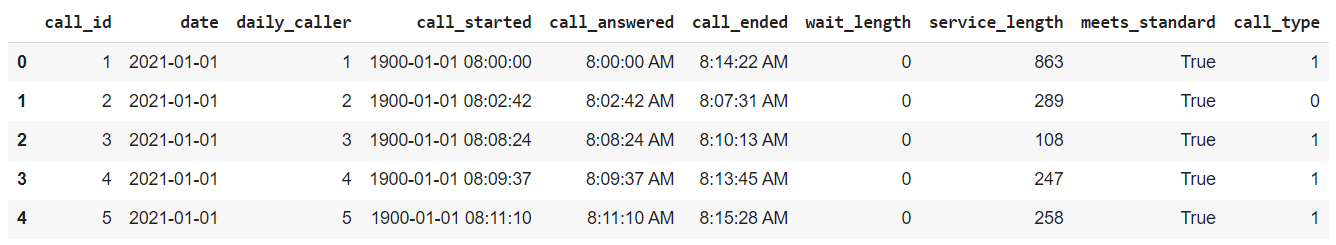
\includegraphics[scale= 0.6]{introducao/imgintro.png}
    \caption{Banco de dados - 5 primeiras chamadas}
    \label{fig: bd_img}
\end{figure}
Na Figura \ref*{fig: bd_img}, pode-se observar 5 ligações registradas dentro da base de dados, bem como todas as variáveis.
\begin{itemize} 
    \item"Call\_id" é a identificação da ocorrência
    \item"date" é a data
    \item "daily\_caller" registra as ligações num dia
    \item"call\_started", "call\_answered" e "call\_ended" são os momentos de ligação, atendimento e término das chamadas
    \item wait\_length é o tempo de espera
    \item"service\_length" é o tempo de atendimento
    \item"meets\_standard" retorna verdadeiro caso o tempo de espera seja menor do que um minuto 
    \item"call\_type" é o tipo da ligação.
\end{itemize}
Para os testes de hipóteses atrelados às diferenças entre essas variáveis em diferentes períodos foi utilizado o método Kolmogorov-Smirnov para duas amostras que possui caráter não parametrico, sendo assim:\\
\begin{center}
$H{0}$ : Amostras seguem a mesma distribuição\\
$H{a}$ : Amostras seguem distribuições diferentes
\end{center}
Posteriormente a confirmação positiva da diferença entre amostras, foi realizado o teste de aderência das amostras às distribuições cauchy, chi quadrado, exponencial, gamma, lognormal, normal, powerlaw, rayleigh, uniforme.\\
Por último para analisar as correlações entre variáveis, foram realizadas regressões lineares e exponeciais.\\

\subsection{Próxima etapa}
Para a próxima etapa do processo, será realizada a modelagem da diferença entre chegadas (ligações) no sistema, para que posteriormente seja desenvolvida a simulação no ARENA.

\subsection{Ferramentas utilizadas}
A modelagem e as análises estatísticas do projeto foram todas realizadas em python 3.9, através do ambiente google colab.\\
Para isso, foram utilizadas as bibliotecas:
\begin{itemize}
    \item pandas
    \item numpy
    \item seaborn
    \item fitter
    \item scipy.stats
    \item tabulate
    \item sklearn.linear\_model
    \item statsmodels.api
    \item scipy.linalg
    \item matplotlib.pyplot
    \end{itemize}